\subsection{Caracterizaci\'on de una soluci\'on}
\begin{itemize}
	\item Una posible soluci\'on es un subconjunto de elementos del conjunto original tal que la suma de ellos es menor al valor objetivo.
	\item Una soluci\'on factible de nuestro problema es un subconjunto de elementos del conjunto original tal que la suma de ellos es exactamente el valor objetivo.
	\item Una soluci\'on no factible es un subconjunto de elementos del conjunto original tal que la suma de ellos es mayor al valor objetivo
\end{itemize}
\subsection{Espacio de soluciones}
En la imagen podemos ver, que luego de diferentes decisiones, llegamos a diferentes soluciones.
\begin{itemize}
	\item Los nodos hojas son las soluciones y est\'an separados en tres casos.
	\item Los nodos celestes son las posibles soluciones.
	\item Los nodos verdes son las soluciones factibles.
	\item Los nodos rojos son las soluciones no factibles. 
\end{itemize}	
\begin{center}
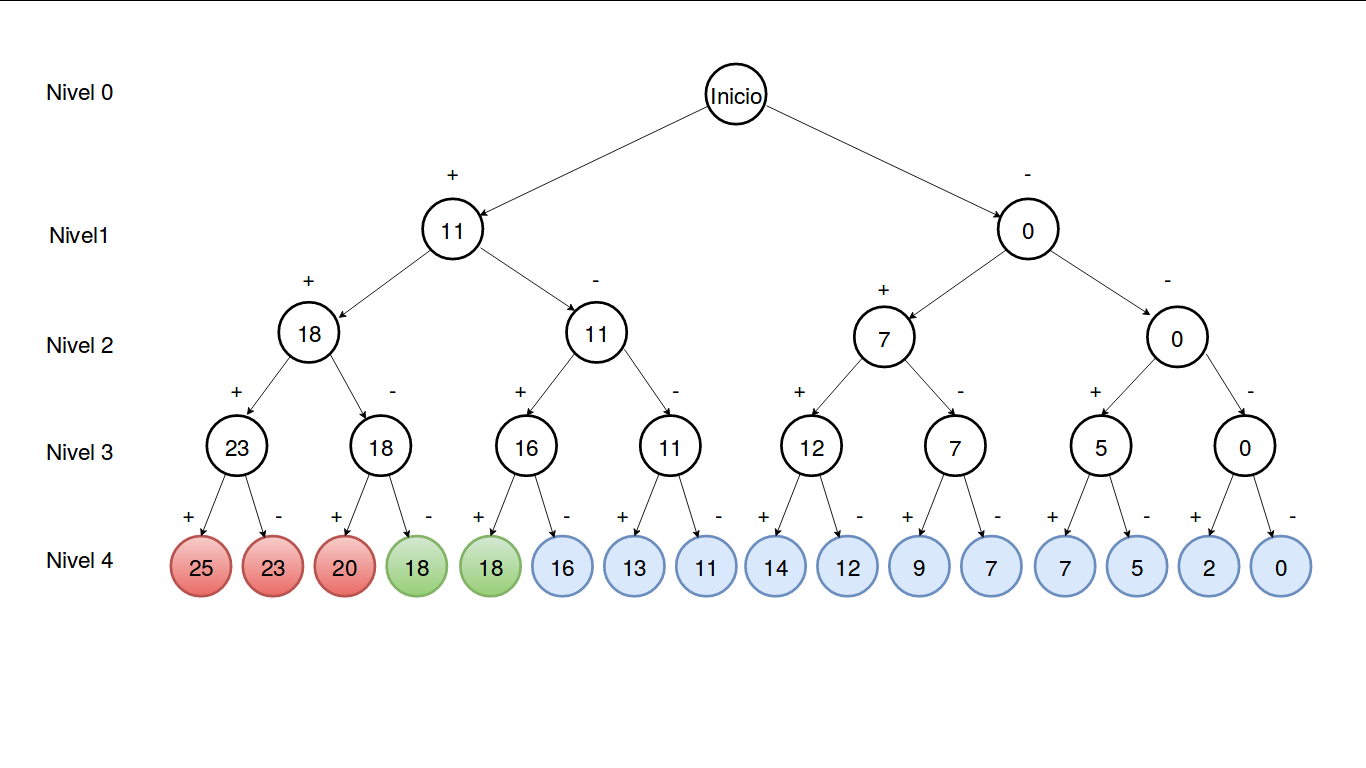
\includegraphics[width=18cm, height=12cm]{3casos.png}
\end{center}
\subsection{Recorrido del espacio de soluciones}
Se ver\'an diferentes formas de pensar el problema, y en base a ello elegiremos una forma de obtener la soluci\'on.\\

\begin{itemize}
\item La primer forma de ver el problema es simple, mirar todo el espacio de soluciones y quedarnos con la mejor.\\
\item En la segunda forma trataremos de recorrer solamente el espacio de posibles soluciones y el espacio de soluciones factibles.\\
\item La tercer forma va mas enfocado a cuando una soluci\'on es mejor que otra, y veremos como recorrer las soluciones que son mejores que la soluci\'on que tenemos hasta el momento(si las hay, sino podaremos).\\
\item La ultima forma de pensar el problema sera ver los problemas anteriores inmediatos y ver como con ellos se puede construir el problema mas grande y gracias a memorizar los subproblemas poder obtener el siguiente de forma eficiente.
\end{itemize}